\documentclass[twocolumn,11pt]{article}
\usepackage[top=1.0in, bottom=1.00in, left=0.5in, right=0.5in]{geometry}
\setlength{\columnsep}{0.35in}
\usepackage{tikz}
\usetikzlibrary{arrows,automata,calc,shapes.symbols,positioning}

\title{scientific writing toolkit - a short (mis)introduction}

\author{https://github.com/pkorus/swtk}

\date{\today}

\begin{document}

\maketitle

\abstract{The sole purpose of this document is to serve as an example of bad writing - an excellent battlefield for the \emph{scientific writing toolkit}. We'll quickly go through some examples of possible pitfalls that endanger your manuscript's clarity, and use them to illustrate existing text analysis modules. For more information (and for the sake of your sanity), refer to more comprehensive, and better written, sources~\cite{strunk}.}
	
\section{Strengthening the Verbs}

This is one of the most common problems. Overusing weak verbs (like "is" or "has") is the cause of your problems. It is boring the reader, making them yawn, and also makes your message unmemorable. It is your duty to maintain his attention. It is also important to remember - your manuscript is supposed to be pleasant to read. It is good when your writing is to the point. There are ways to deal with it, though.

Keeping this in mind, make sure to use strong verbs. Engage the reader; grip his attention early - never let go :) Be succinct. Dispense with redundant clutter and confounding doublespeak. Convey your message clearly. Good writing helps your "take home message" be memorable. Adapt to your readership. 

\section{Verb Excavation}

\emph{Buried verbs}, you know, the ones that are far, really far, far away from the subject, make your text really insufferable. A recent large-scale analysis of 37 diverse languages, performed by scholars from MIT, and published not very long ago in the Proceedings of the National Academy of Sciences of the United States of America, provides evidence that the \emph{dependency length} tends to be minimized across many languages~\cite{dlm}. The term, being more general than just a subject-verb property - and I am really glad you made it this far in this paragraph - refers to syntactically related words. At this point, you should have been doubtlessly convinced that sentences with long dependencies are more difficult to read. So make your readers a solid, and keep the scientific writing toolkit close, and your subjects and verbs closer. 

\section{Hunting Clutter}

This section provides a review that is based on enumeration of unnecessary words and phrases and words. Very often, one could even say typically, your first draft will be scattered with unnecessary clutter. There are many words you could have used for this purpose. There are two primary suspects that are typically probably guilty of making your writing weak and without strength. The list includes, but is not limited to, two items listed below in an itemization environment which serves only the purpose of showing you that the scientific writing toolkit can indeed support itemization environments, even though only not nested ones are properly handled: 

\begin{itemize}
	\item \emph{verbs transmogrified into nouns},
	\item \emph{vague adverbs}.
\end{itemize}

The first wrongdoing culprit is based on production of sentences where a supposedly smart-looking noun (like "enumeration" or "review") that most likely is a nice strong verb is an alternative realty where your writing does not suck. In that better (although probably not yet perfect) reality, this section has most likely started with a statement like: "This section reviews and enumerates unnecessary words and phrases that often run rampant in your first draft."

\begin{figure}
\centering
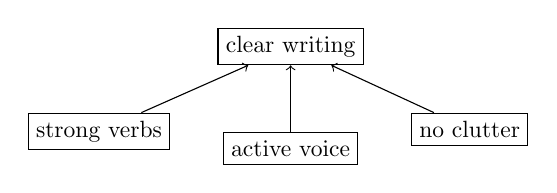
\begin{tikzpicture}[scale=0.85,transform shape]
\node[draw] (root) {clear writing};
\node[draw,below left=1 of root] (leaf) {strong verbs}; \path[draw,->] (leaf) edge (root);
\node[draw,below= of root] (leaf) {active voice}; \path[draw,->] (leaf) edge (root);
\node[draw,below right=1 of root] (leaf) {no clutter}; \path[draw,->] (leaf) edge (root);
\end{tikzpicture}
\caption{There are also figures that can be clutter. The purpose of this figure is to perform introduction of no new information to this document. And maybe to show you that captions of the figures can be included in your report. While we're at it, $\sum_{i=1}^{\infty}\frac{1}{2^n}=\frac{1}{2} + \frac{1}{4} + \ldots$.}
\end{figure}

Typically, the second unwanted garbage in your shiny new manuscript is probably an epidemic-like event that causes a presence of totally unnecessary vague adverbs that doubtlessly are vague and meaningless and are possibly and actually not needed where they are. While sometimes you can use adverbs occasionally, make sure to usually keep their population-based property to minimum. Totally!

\section{Staying Active}

While most journals are far enough from adopting corporal punishment for using passive voice, it should be kept in mind that words are typically spoken in active voice. Such sentences are simply more natural to parse. It is rather expected by people that the sentence is begun with a subject, and the subject is followed by a verb. My words are not to be misunderstood here. Passive voice is to be used. But it is to be used thoughtfully. And from time to time, your mind should be crossed by a simple question - wouldn't this sentence be clearer if it were written in a way that the words are usually put in?

\begin{thebibliography}{50}
\bibitem{strunk}{W. Strunk Jr., The Elements of Style, http://www.gutenberg.org/ebooks/37134}
\bibitem{dlm}{Richard Futrell, Kyle Mahowald, and Edward Gibson, Large-scale evidence of dependency length minimization in 37 languages, Proc. of the National Academy of Sciences of the United States of America, http://www.pnas.org/content/112/33/10336}
\end{thebibliography}
	
\end{document}